% !TeX spellcheck = en_GB
\documentclass[preprint,authoryear]{elsarticle}

\usepackage{natbib}
\bibliographystyle{elsarticle-harv}

\usepackage{algorithm}
\usepackage{algpseudocode}

\usepackage{amsmath,amsthm}
\usepackage{amssymb}

\usepackage[latin1]{inputenc}
\usepackage[T1]{fontenc}

\usepackage{multirow}

\usepackage[none]{hyphenat}

\usepackage{booktabs}

\usepackage{tikz}
\usetikzlibrary{calc}
\usetikzlibrary{positioning}

\usepackage{caption}
\captionsetup{labelfont=bf}
\captionsetup{skip=0pt}

\usepackage{pgfplots}
\pgfplotsset{compat=newest}

\newcommand{\boldm}[1] {\mathversion{bold}#1\mathversion{normal}}
\newcommand{\round}[1]{\ensuremath{\lfloor#1\rceil}}

\usepackage{color, colortbl}

\definecolor{Gray}{gray}{0.9}
\hyphenation{cost-ef-fec-tive-ness}

\usepackage{setspace} 

\newcommand{\specialcell}[2][c]{%
	\begin{tabular}[#1]{@{}c@{}}#2\end{tabular}}

\usepackage[margin=2.3cm]{geometry}
\geometry{a4paper}


\journal{Expert Systems with Applications}

\begin{document}

\begin{frontmatter}
	
	\title{Air cargo load and route planning in pickup and delivery operations}
	
	\author{A.C.P.~Mesquita}
	\ead{celio@ita.br}
	
	\author{C.A.A.~Sanches\corref{cor1}}
	\ead{alonso@ita.br}
	\cortext[cor1]{Corresponding author.}
	
	\address {Instituto Tecnol\'{o}gico de Aeron\'{a}utica - DCTA/ITA/IEC\\
		Pra\c{c}a Mal. Eduardo Gomes, 50\\
		S\~{a}o Jos\'{e} dos Campos - SP - 12.228-900 - Brazil}


\begin{abstract}
In the aerial pickup and delivery of goods in a distribution network, transport aviation faces risks of load imbalance due to the urgency required for loading, immediate take-off, and mission accomplishment. Transport planners deal with trip itineraries, prioritisation of items, building up pallets, and balanced loading, but there are no commercially available systems that can integrally assist in all these requirements. This enables other risks, such as improper delivery, excessive fuel burn, and possible safety issues due to cargo imbalance, as well as a longer than necessary turn-around time.�This {\it NP-hard}\/ problem, named {\it Air Cargo Load Planning with Routing, Pickup, and Delivery Problem (ACLP+RPDP)}, is mathematically modelled using standardised pallets in fixed positions. We developed a strategy to solve this problem, considering historical transport data from some Brazilian hub networks, and performed several experiments with a commercial solver, four known meta-heuristics, and a new heuristic designed specifically for this problem. By using a portable computer, our strategy quickly found practical solutions to a wide range of real problems in much less than operationally acceptable time.
\end{abstract}

\begin{keyword}
	OR in Airlines \sep Load Planning \sep Air Palletization \sep Weight and Balance \sep Pickup and Delivery \sep Vehicle Routing
\end{keyword}

\end{frontmatter}



\section{Introduction}\label{sec:Introduction}

The aviation industry adapts during global crises to keep supply chains moving. Air cargo provided complex expertise and the ability to access diverse destinations, delivering essential goods such as medicines, vaccine supplies, testing kits and other necessities with exceptional speed. This mode of transportation has become a preferred choice for governments, corporations and global companies in urgent need of transportation solutions.

Air cargo services are specially designed for organisations that require customised transportation, handle sensitive goods, or serve remote locations with limited routes. Air carriers typically use high-capacity cargo planes for economies of scale. Many cargo airlines have worldwide networks spread across destinations around the world.

Recently, \citep{BrandtStefan2019} defined the {\it Air Cargo Load Planning Problem} (ACLPP) as four sub-problems: {\it Aircraft Configuration Problem} (ACP), {\it Build-up Scheduling Problem} (BSP), {\it Air Cargo Palletization Problem} (APP), and {\it Weight and Balance Problem} (WBP). Several aspects were considered: item characteristics to be transported (dimensions, scores, dangerousness, etc.); types and quantities of {\it unit load devices} (ULDs); when these pallets are assembled; how items are allocated to pallets; in which positions these pallets are to be placed; how total cargo weight is balanced; etc.

However, it is crucial to highlight that there are still other important challenges in air cargo transport that go beyond the definition of ACLPP, especially with regard to routes, and pickup and delivery at each destination. In this context, at least two more important sub-problems can be considered: simultaneous pickup and delivery at each node, called the {\it Pickup and Delivery Problem} (PDP), and searching for the best benefit-cost route, which is a special case of the {\it Travelling Salesman Problem} (TSP).

The problem addressed in this work is the definition of the route of an aircraft that loads and unloads hundreds of items in up to seven hubs, dealing with weight, volume, and balance constraints, and maximising the benefit-cost ratio. This challenge has become even more acute during the COVID-19 pandemic due to the need for urgent medical supplies. Delays in shipping essential items such as respirators to critical areas highlighted the need for optimised solutions.

This problem is extremely complex, as it deals with different objectives: defining a route that visits all hubs; maximising the items transported along this route, prioritising the essential ones; making sure items reach the correct destinations; ensuring aircraft safety constraints; and saving fuel so that the flight is sustainable. 

We have developed a heuristic process that can be run on a handheld computer, quickly providing a good solution to real instances of this problem. Solutions consist of flight itineraries, pickup and delivery plans, and the allocation of items onto pallets, ensuring the load-balancing constraints. Our method also reduces the stresses that transport planners are subject to, as they have to deal with extensive information in a short time frame.

To the best of our knowledge, this is the first time that an air cargo problem involving simultaneously APP, WBP, PDP, and TSP has been addressed. This new problem is named {\it Air Cargo Load Planning with Routing, Pickup, and Delivery Problem} (ACLP+RPDP). As we will describe in our mathematical modelling, these four sub-problems appear in an interconnected way in ACLP+RPDP and therefore cannot be solved independently.

As a real case study, we consider a crucial network for the {\it Brazilian Air Force}, as can be seen in Table \ref{tab:costs} and Figure \ref{fig:nodes}. Although there are other airports of interest, these nodes were chosen due to their high demand. Other Brazilian airports tend to have smaller transport requests, which are generally met less expensively by cabotage, rail, or road transport.

\begin{table}[htb]
	
	\begin{minipage}{0.58\linewidth}
		
		\caption{Brazilian airports distances ($km$)} \label{tab:costs}
		\centering
		\footnotesize
		
		\newcolumntype{C}{>{\centering\arraybackslash}p{0.07\textwidth}}
		\newcolumntype{R}{>{\raggedleft\arraybackslash}p{0.07\textwidth}}			
		
		\begin{tabular}{C R R R R R R R}
			\toprule
			IATA*   & GRU   & GIG   & SSA   & CNF   & CWB   & BSB   & REC \\	
			\midrule	
			GRU     & 0	    &343	&1,439   &504    &358    &866    &2,114\\
			GIG	    & 343	&0	    &1,218   &371    &677    &935    &1,876\\
			SSA	    & 1,439	&1,218	&0	    &938    &1,788   &1,062   &676\\
			CNF	    & 504	&371	&938	&0	    &851    &606    &1,613\\
			CWB	    & 358	&677	&1,788	&851	&0	    &1,084   &2,462\\
			BSB	    & 866	&935	&1,062	&606	&1,084	&0	    &1,658\\
			REC	    & 2,114	&1,876	&676	&1,613	&2,462	&1,658	&0\\
			\bottomrule
			\multicolumn{8}{c}{*International Air Transport Association}\\
			\multicolumn{8}{c}{\small\textsuperscript{Source: www.airportdistancecalculator.com}}\\
		\end{tabular}
		\normalsize
		
	\end{minipage}\hfill 
	\begin{minipage}{0.42\linewidth}
		\centering
		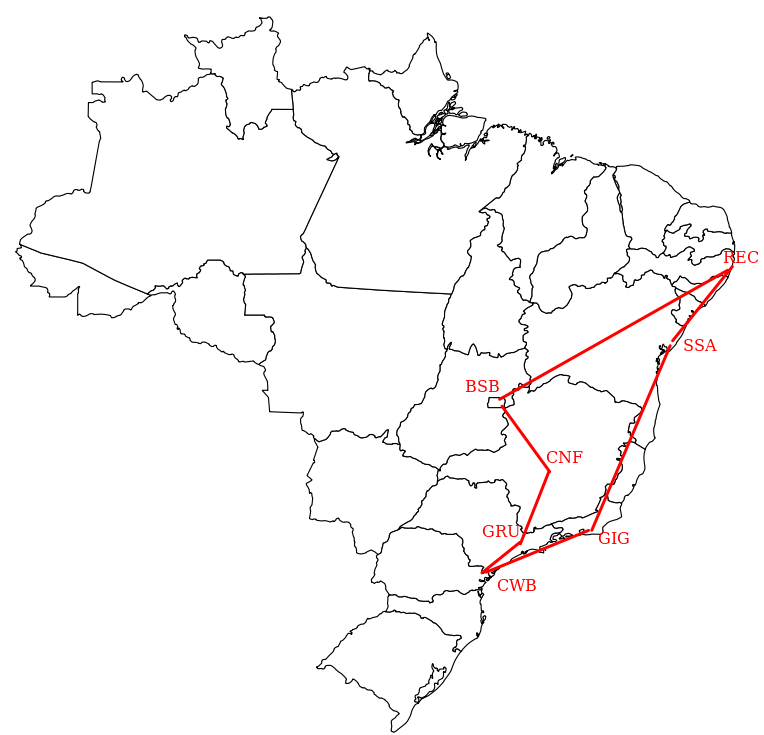
\includegraphics[scale=0.17]{nodes.png}
		\captionof{figure}{A route with 7 airports}
		\label{fig:nodes}
	\end{minipage}
\end{table}

This article is organised into six more sections. In Section \ref{literature}, we make the literature review. In Section \ref{assumptions}, we present the context and requirements of ACLP+RPDP. In Section \ref{modelling}, we describe its mathematical modelling. In Section \ref{algorithms}, we describe the developed algorithms, whose results are presented in Section \ref{results}. Finally, our conclusions are in Section \ref{conclusions}.

\section{Literature review}
\label{literature}

The vast majority of operational research applied to air cargo is focused on challenges related to WBP, that is, the distribution of items on pallets to ensure load balancing. We can mention: \citep{LarsenMikkelsen1979}; \citep{Brosh1981}; \citep{Kevin1992}; \citep{Heidelberg1998}; \citep{fok2004optimizing}; \citep{KaluznyBohdanL2009Oalb}; \citep{Verstichel2011}; \citep{Limbourg2012}; \citep{RoesenerBarnes2016}; \citep{YangLiuGao2018}; \citep{zhao2021}; \citep{MiguelOptimalAP}.

Other authors have addressed pallet assembly (APP) on aircraft, possibly also considering load balancing (WBP): \citep{MongeauBes2003}; \citep{Chan2006}; \citep{RoesenerHall2014}; \citep{Vancroonemburg2014}; \citep{Paquay2016}; \citep{Paquay2018}; \citep{wong2020}; \citep{eugene2021}; \citep{zhao2023}.

In all these works, there is a great diversity of scenarios and solutions: some consider items in two dimensions, and others in three dimensions; some used integer programming, and others developed specific heuristics.

\citep{LurkinSchyns2015} is the only work that simultaneously addresses an air cargo (WBP) and a flight itinerary (PDP) sub-problem. The authors demonstrated that this problem is {\it NP-hard}. Although it is innovative, strong simplifications were imposed by these authors: in relation to loading, APP was ignored; regarding routing, it is assumed that a predefined tour plan is restricted to only two legs. Referring directly to this work, \citep{BrandtStefan2019} comment: {\it However, not even these sub-problems are acceptably solved for real-world problem sizes, or models omit some practically relevant constraints}.

Table \ref{tab:sa} lists this literature and the involved sub-problems. We also indicate whether the dimensions of the items were considered ({\bf 2D} or {\bf 3D}) and which solution method was used: heuristic search methods ({\bf Heu}), integer programming ({\bf Int}), or linear programming ({\bf Lin}).

\begin{table}[h]
	\centering
	\caption{Air cargo transport: literature, sub-problems and features}  \label{tab:sa}
	\footnotesize
	\begin{tabular}{r|cccc|ccccc}
		\toprule
		Work & {\bf APP}  & {\bf WBP}  &  {\bf PDP}   &{\bf TSP}   & {\bf 2D}  & {\bf 3D}  & {\bf Heu}  & {\bf Int}  & {\bf Lin} \\
		\midrule
		\citep{LarsenMikkelsen1979}  & $.$        & $\bigstar$ & $.$          & $.$        & $.$       & $.$       & $\bigstar$ & $.$        &  $.$ \\
		\citep{Brosh1981}  & $.$ & $\bigstar$  & $.$   & $.$ & $.$ & $.$   & $.$  & $.$  &  $\bigstar$ \\
		\citep{Kevin1992}  & $.$ & $\bigstar$  & $.$ & $.$ & $.$ &$.$   & $.$  & $\bigstar$  &  $.$ \\
		\citep{Heidelberg1998}  & $.$ & $\bigstar$  & $.$ & $.$ & $\bigstar$ &$.$   & $\bigstar$  & $.$  &  $.$ \\
		\citep{MongeauBes2003}    & $\bigstar$ & $\bigstar$   & $.$ & $.$ & $.$ & $.$   & $.$  & $\bigstar$  &  $.$ \\
		\citep{fok2004optimizing} & $.$ & $\bigstar$   & $.$ & $.$ & $.$ & $.$   & $.$  & $\bigstar$  &  $.$ \\	
		\citep{Chan2006}  & $\bigstar$ & $.$    & $.$ & $.$ & $.$ & $\bigstar$  & $\bigstar$  & $.$  &  $.$ \\
		\citep{KaluznyBohdanL2009Oalb}  & $.$ & $\bigstar$  & $.$  & $.$ & $\bigstar$ &$.$  & $.$  & $\bigstar$  &  $.$ \\
		\citep{Verstichel2011}   & $.$ & $\bigstar$    & $.$ & $.$ & $.$ & $.$   & $.$  & $\bigstar$  &  $.$ \\	
		\citep{Limbourg2012} & $.$ & $\bigstar$  & $.$ & $.$ & $.$ & $.$   & $.$  & $\bigstar$  &  $.$ \\
		\citep{RoesenerHall2014}  & $\bigstar$ & $\bigstar$  & $.$  & $.$ & $.$ & $\bigstar$   & $.$  & $\bigstar$  &  $.$ \\
		\citep{Vancroonemburg2014}  & $\bigstar$ & $\bigstar$   & $.$ & $.$ & $.$ & $.$   & $.$  & $\bigstar$  &  $.$ \\
		\citep{LurkinSchyns2015} & $.$ & $\bigstar$  & $\bigstar$ & $.$  & $.$ & $.$   & $.$  & $\bigstar$  &  $.$ \\
		\citep{RoesenerBarnes2016}  & $.$ & $\bigstar$   & $.$ & $.$ & $.$ & $.$   & $\bigstar$  & $.$  &  $.$ \\
		\citep{Paquay2016,Paquay2018}  & $\bigstar$ & $\bigstar$ & $.$ & $.$ & $.$ & $\bigstar$ & $\bigstar$  & $\bigstar$ & $.$ \\
		\citep{YangLiuGao2018} & $.$ & $\bigstar$  & $.$  & $.$ & $\bigstar$  & $.$ & $\bigstar$ & $.$  & $.$ \\
		\citep{wong2020} & $\bigstar$  & $\bigstar$  & $.$  & $.$   & $.$  & $.$ & $.$ & $\bigstar$  & $.$  \\
		\citep{eugene2021} & $\bigstar$ & $\bigstar$ & $.$  & $.$   & $.$ & $.$ & $.$ & $\bigstar$  & $.$  \\
		\citep{zhao2021} & $.$ & $\bigstar$ & $.$  & $.$  & $.$ & $.$ & $.$  & $\bigstar$ &  $.$ \\
		\citep{zhao2023} & $\bigstar$ & $\bigstar$ & $.$  & $.$  & $.$ & $.$ & $.$  & $\bigstar$ &  $.$  \\
		\citep{MiguelOptimalAP} & $.$ & $\bigstar$ & $.$  & $.$  & $.$ & $.$ & $.$  & $\bigstar$ &  $.$  \\
		{\bf This article}   & $\bigstar$ & $\bigstar$  & $\bigstar$& $\bigstar$ & $.$ & $.$ & $\bigstar$ & $\bigstar$   &  $.$  \\
		\bottomrule 
	\end{tabular}
	\normalsize 
\end{table}

As can be seen, none of these papers address air cargo palletization and load balancing with route optimisation in a multi-leg transport plan for a single aircraft. Our work is the first to address a real air transport problem in which APP, WBP, PDP and TSP arise in an interconnected way.

\section{Context and assumptions}
\label{assumptions}

In this section, we describe the context of the problem addressed in this work as well as the assumptions considered.

{\color{blue}

As for the size of the problem dealt with in this work, addressing the scale of the Travelling Salesperson Problem (TSP) in practical, real-world air transport contexts indeed reveals a fascinating and complex challenge. In the realm of academic research, TSP problems often explore theoretical models that can scale to hundreds or even larger numbers of cities.

In practical terms, especially within the air transport sector, the size and complexity of a TSP can vary significantly depending on several factors:

\textbf{Fleet and Route Planning}: For airline operations, the problem isn't just about finding the shortest path through a set of points but also involves scheduling, aircraft assignment, crew scheduling, and maintenance planning. This multi-dimensional complexity transforms a standard TSP into a more intricate problem in our study, the Pickup and Delivery Problem (PDP).

\textbf{Operational Constraints}: Factors like weather, air traffic control restrictions, and the availability of take-off and landing slots make real-world TSP scenarios in air transport even more challenging. These constraints add layers of complexity that significantly depart from the theoretical TSP model.

\textbf{Dynamic Nature}: Unlike the static nature of classical TSP, real-world problems in air transport are highly dynamic. Routes need to be optimized continuously as conditions change, requiring algorithms that can adapt in real-time or near-real-time.

In practical air transport scenarios, the size of a TSP can be less about the sheer number of nodes and more about the complexity and dynamic nature of the problem, which in our case (a single aircraft in a single day) is rarely expected to be more than seven nodes. Despite this, at the end of this work, we intend to submit the best method found to a more challenging 15-node problem as a validation test.
}

\subsection{Operational premises}

As we are dealing with an extremely complex and diverse problem, we decided to establish some simplifying characteristics:

\begin{itemize}
	\setlength\itemsep{-0.3em}
	
	\item At each node of the tour, the items to be allocated are characterized by weight, volume, scores, and previously known destinations. We leave the consideration of 2D or 3D items to a future work.
	
	\item We considered a unique pallet type: the {\it 463L Master Pallet}, a common size platform for bundling and moving air cargo. It is the primary air cargo pallet for more than 70 Air Forces and many air transport companies. This pallet has a capacity of $4,500 kg$ and $13.7 m^3$, which may be limited by its position along the cargo bay. It is equipped for locking into cargo aircraft rail systems, and includes tie-down rings to secure nets and cargo loads, which in total weighs $140 kg$. For more information, see {\tt www.463LPallet.com}.
	
	\item All items allocated on a pallet must have the same destination. A pallet which has not yet reached its destination may receive more items, although it is known that these operations of removing restraining nets increase handling time and the risk of improper delivery. We do not consider oversized cargo in this work, but only cargo items that fit on these pallets.
	
	\item Finally, as we are interested in minimizing fuel costs, we disregarded others costs not directly associated with aircraft flight, such as handling.
	
\end{itemize}

Throughout this text, we call {\it packed content}\/ a set of items of the same destination stacked on a pallet and covered with a restraining net. It is considered a single item, having the same attributes as its components, whose values are the sum of individual scores, weights, and volumes. To ensure accuracy in pickup and delivery operations, packed content must remain on board until its destination.


\subsection{Aircraft parameters and load balancing}

We consider real-world scenarios, where Table \ref{tab:larger} shows the aircraft parameters. $p_i$\/ are pallets, $1\leq i \leq 18$, whose weight and volume limits are $W_i$\/ and $V_i$, respectively. $D_i^{long}$\/ and $D_i^{lat}$\/ are, respectively, the longitudinal and lateral distances of each pallet centroids to the aircraft centre of gravity (CG) along both axes. These distances will be used in the calculation of the torque, referring to the items allocated on each pallet. In this aircraft, as the ramp has an inclination of $25^{\circ}$, we made the necessary corrections in $D_i^{long}$, $W_i$\/ and $V_i$\/ of the corresponding pallets ($p_1$, $p_2$, $p_3$, and $p_4$).




\begin{table}[h]
	\centering
	\caption{Aircraft parameters}  \label{tab:larger}
	\footnotesize
	\begin{tabular}{c | c c c c c c c c c}
		\toprule
		& \multicolumn{3}{c}{$Payload$: 75,000kg} & \multicolumn{3}{c}{$limit^{CG}_{long}$: $1.170m$} &
		\multicolumn{3}{c}{$limit^{CG}_{lat}$: $0.19m$} \\
		\midrule
		\multirow{2}{*}{{\boldm{$p_i$}}}  & $p_{17}$ & $p_{15}$ & $p_{13}$ & $p_{11}$ & $p_{9}$ & $p_{7}$ & $p_{5}$ & $p_{3}$ & $p_{1}$ \\
		& $p_{18}$ & $p_{16}$ & $p_{14}$ & $p_{12}$ & $p_{10}$ & $p_{8}$ & $p_{6}$ & $p_{4}$ & $p_{2}$ \\
		\midrule 
		\multirow{2}{*}{\boldm{$D_i^{long}$} ($m$)} & -17.57 & -13.17 & -8.77 & -4.40 & 0 & 4.40 & 8.77 & 11.47 & 14.89 \\
		& -17.57 & -13.17 & -8.77 & -4.40 & 0 & 4.40 & 8.77 & 11.47 & 14.89 \\			
		\midrule 
		\multirow{2}{*}{\boldm{$D_i^{lat}$} ($m$)}  & 1.32 & 1.32 & 1.32 & 1.32 & 1.32 & 1.32 & 1.32 & 1.32 & 1.32 \\
		& -1.32 & -1.32 & -1.32 & -1.32 & -1.32 & -1.32 & -1.32 & -1.32 & -1.32 \\	
		\midrule
		{\boldm{$W_i$}} ($kg$)      &   4,500   &    4,500  &   4,500   &  4,500    & 4,500     & 4,500     & 4,500     & 3,000    & 3,000   \\
		{\boldm{$V_i$}} ($m^3$)   &   14.8   &   14.8   &  14.8    &  14.8    & 14.8     & 14.8     & 14.8     & 10.0    & 7.0 \\	
		\midrule	
		\textbf{Fuel cost}  & \multicolumn{9}{c}{ $c_d$ = US\$ $4.90/km$ }	 \\
		\midrule
		\textbf{Fuel consumption rate}  & \multicolumn{9}{c}{ $c_g = 5\%$} \\		
		\midrule
		\textbf{Maximum weight}  & \multicolumn{9}{c}{ $W_{max} = \sum_i W_i = 75,000kg$} \\
		\bottomrule
	\end{tabular}
	\normalsize 
\end{table}


This aircraft spends $c_d$\/ dollars per kilometre flown and can carry up to $W_{max}$\/ of cargo distributed on the pallets. The fuel penalty $c_g$\/ is the percentage of cost increase due to the CG deviation on the longitudinal axis, estimated at 5.0\%. It is important to consider that $c_g$\/ tends to zero as the aircraft attitude tends to be level. As the CG deviation varies from $0$\/ to $limit^{CG}_{long}$, this fuel penalty varies from $0$\/ to $c_g$.

The torque applied to the aircraft must keep its CG in the operational range, which corresponds to a fixed percentage of the {\it Mean Aerodynamic Chord} \footnote{Chord is the distance between the leading and trailing edges of the wing, measured parallel to the normal airflow over the wing. The average length of the chord is known as the {\it Mean Aerodynamic Chord} (MAC).} which is considered $1.17m$ for the aircraft of this work (see Figure \ref{fig:lateral}).


\begin{figure}[h]
	\centering
	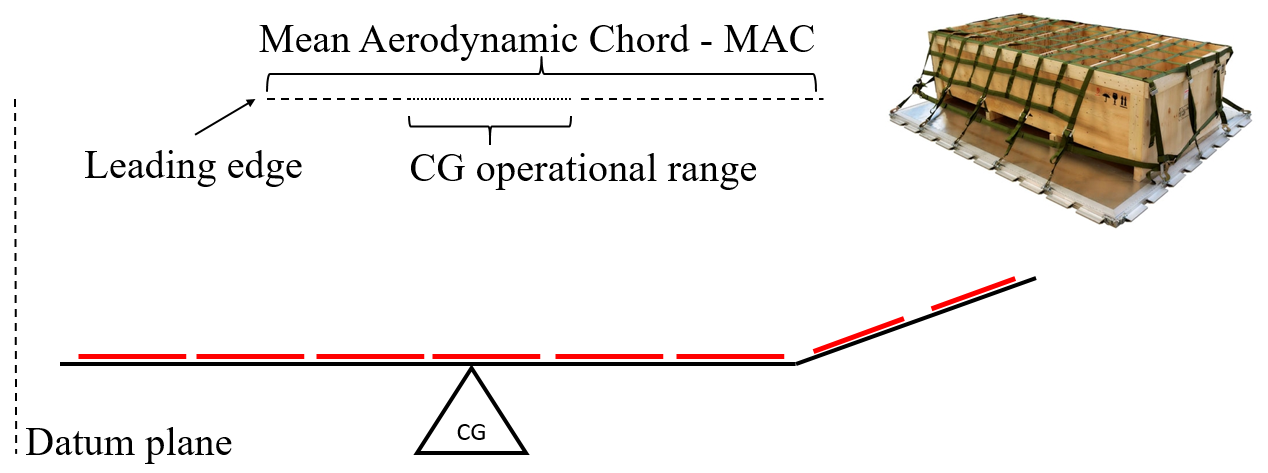
\includegraphics[scale=0.22]{lateral.png}
	\caption{Aircraft longitudinal cut, where red lines are pallets positions}
	\label{fig:lateral}
\end{figure}


We also make the following assumptions:

\begin{itemize}
	\setlength\itemsep{-0.3em}
	\item on each pallet, the items are distributed in such a way that their CG coincides with the centroid of the pallet, because builders are well-trained to do so;
	\item the CG of the total load must be at a maximum longitudinal distance of $limit^{CG}_{long}$\/ from the CG of the aircraft;
	\item the CG of the total load must be at a maximum lateral distance of $limit^{CG}_{lat}$\/ from the CG of the aircraft;
	\item the pallets are distributed in two identical rows (with odd and even indices, respectively), and the centroid of $p_i$\/ is at a distance $D^{lat}_{i}$\/ from the centreline of the aircraft;
	\item when there are items or packed contents in $p_i$, the common destination of this load will be assigned to variable $T_i$. 
\end{itemize}


\section{The mathematical modelling}
\label{modelling}


In this section, we present the mathematical modelling of ACLP+RPDP in Tables \ref{tab:struc}, \ref{tab:graph}, \ref{tab:functions}, and \ref{tab:constraints}, with their corresponding descriptions.

In Table \ref{tab:struc}, we describe the problem structure: nodes and their permutations, distances and associated costs, pallets characteristics, items available for shipment at each node, and packed contents shipped. The item $j$\/ in node $k$\/ has score $s_j$, weight $w_j$, volume $v_j$, and destination $to_j \in L_k$. Similarly, the packed content $q$, that remains on board at node $k$, has total weight $w_q$, total volume $v_q$, and destination $to_q \in L_k$. Packed contents that were destined to node $k$\/ are unloaded when the aircraft arrives there; that is, they are not considered in $Q_k$.

\begin{table}[ht]
	\centering
	\footnotesize
	\caption{Problem structure}  \label{tab:struc}
	\begin{tabular}{l l}
		\toprule
		\textbf{Notation}	& \textbf{Description} \\
		\midrule
		$L = \{ 0, 1, \ldots, K \}$ & Set of $K+1$\/ nodes of the tour, where node 0 is the base \\
		\midrule
		$\pi$               & A permutation between nodes 1, \ldots, $K$\\
		\midrule
		$S_K$               & Set of $K!$\/ permutations \\
		\midrule
		$\pi_k$             & The $k^{th}$\/ node of tour $\pi$, $1 \leq k \leq K$\\
		\midrule
		Tour $\pi$          & $\{0,\pi_1,\ldots, \pi_K, 0\}$ \\
		& For ease of notation, $\pi_0 = \pi_{K+1} = 0$\\
		\midrule
		$L_k$               & Set of remaining nodes of tour at node $k$, $0 \leq k \leq K$\\
		& By definition, $L_0 = L$\\
		\midrule
		$d(a,b)$            & Distance from node $a$\/ to node $b$, where $0 \leq a, b \leq K$ \\
		&   By definition, $d(a,a) = 0, \forall a$\\
		\midrule
		$C=\left[c_{a,b}\right]$    & Cost matrix of flights, where $c_{a,b} = c_d \times d(a,b)$\\
		\midrule
		$M = \{1, \ldots, m \}$  & Set of $m$\/ pallets in specific positions within the aircraft \\
		&  See Table \ref{tab:larger}, where $m=18$ \\
		\midrule
		$N_k = \{1, \ldots, n_k \}$ & Set of $n_k$\/ items available for loading at node $k$, $1 \leq j \leq n_k$, $0 \leq k \leq K$\\
		\midrule
		$N = \bigcup_{0 \leq k \leq K} N_k$ & Set of items in all nodes along a tour\\
		\midrule
		$Q_k = \{1, \ldots, m_k \}$ & Set of $m_k \leq m$\/ packed contents at node $k$, $1 \leq q \leq m_k$, $0 \leq k \leq K$ \\ 
		& By definition, $m_0 = 0$ and $Q_0 = \varnothing$\\
		\bottomrule
	\end{tabular}
	\normalsize
\end{table}


Table \ref{tab:graph} contains decision variables and the ACLP+RPDP allocation graph.

\begin{table}[H]
	\centering
	\footnotesize
	\caption{Decision variables and allocation graph}  \label{tab:graph}
	\begin{tabular}{l l}
		\toprule
		\textbf{Notation}	& \textbf{Description} \\
		\midrule
		$X_{ij}^{\pi_k}$\/ and $Y_{iq}^{\pi_k}$ & Binary variables, where $1 \leq i \leq m$, $1 \leq j \leq n_{\pi_k}$, $1 \leq q \leq m_{\pi_k}$\/ and $0 \leq k \leq K$\\
		\midrule
		$X_{ij}^{\pi_k} = 1$ & If item $j$\/ at node ${\pi_k}$\/ is assigned to pallet $i$, and 0 otherwise\\
		\midrule
		$Y_{iq}^{\pi_k} = 1$ & If packed content $q$\/ at node ${\pi_k}$\/ is assigned to pallet $i$, and 0 otherwise\\
		\midrule
		$T_i^{\pi_k} \in L_{\pi_k}$ &  Destination of items and packed contents assigned to pallet $i$\ at node ${\pi_k}$\\
		\midrule
		$G_{\pi_k}(V_{\pi_k}, E_{\pi_k})$ & Allocation graph at node ${\pi_k}$\\
		\midrule
		$V_{\pi_k} = M \cup N_{\pi_k} \cup Q_{\pi_k}$ & Allocation graph vertices at node ${\pi_k}$: pallets, items and packet contents\\
		\midrule
		$E_{N_{\pi_k}}$ & Allocation graph edges at node ${\pi_k}$, corresponding to shipped items\\
		\midrule
		$E_{Q_{\pi_k}}$ & Allocation graph edges at node ${\pi_k}$, corresponding to packed contents\\
		\midrule
		$E_{\pi_k} = E_{N_{\pi_k}} \cup E_{Q_{\pi_k}}$ & Allocation graph edges at node ${\pi_k}$\\
		\midrule
		$(i, j) \in E_{N_{\pi_k}}$ & If $X_{ij}^{\pi_k} = 1$, where $i$\/ is a pallet and $j$\/ is a item at node ${\pi_k}$ \\
		\midrule
		$(i, q) \in E_{Q_{\pi_k}}$ & If $Y_{iq}^{\pi_k} = 1$, where $i$\/ is a pallet and $q$\/ is a packed content at node ${\pi_k}$\\
		\bottomrule
	\end{tabular}
	\normalsize
\end{table}


The calculus functions of ACLP+RPDP are described in Table \ref{tab:functions}.

\begin{table}[H]
	\centering
	\footnotesize
	\caption{Calculus functions} \label{tab:functions}
	\begin{tabular}{ c l }
		\toprule
		\textbf{Function} & \textbf{Description} \\
		\midrule
		(\ref{eq:scores}) & Total score of transported items throughout tour $\pi$\\
		\midrule
		(\ref{eq:tau})    & Longitudinal torque applied by loaded pallets at node ${\pi_k}$\\
		\midrule
		(\ref{eq:costs})  & Total cost of fuel on tour $\pi$\/ (distances and CG longitudinal deviations) \\
		\midrule
		(\ref{eq:departing}) & Set of not visited nodes at node ${\pi_k}$\\
		\midrule
		(\ref{eq:LatItem}) & Lateral torque at node ${\pi_k}$ (shipped items) \\
		\midrule
		(\ref{eq:LatPacked}) & Lateral torque at node ${\pi_k}$ (packed contents)\\
		\midrule
		(\ref{eq1}) & Objective function of ACLP+RPDP\\
		\bottomrule
	\end{tabular}
	\normalsize
\end{table}

\begin{equation} \label{eq:scores}
	\tilde{s}_\pi = \sum_{k=0}^{K} \sum_{i=1}^{m} \sum_{j=1}^{n_{\pi_k}} X_{ij}^{\pi_k} \times s_j
\end{equation}

\begin{equation} \label{eq:tau}
	\tau_{\pi_k} = \sum_{i=1}^{m} \Big [ D_i^{long} \times \Big ( \sum_{j=1}^{n_{\pi_k}} X_{ij}^{\pi_k} \times w_j +  \sum_{q=1}^{m_{\pi_k}} Y_{iq}^{\pi_k} \times w_q \Big ) \Big ] \Big / W_{max} \times limit^{CG}_{long}; \ k \in \{0, \ldots, K\}
\end{equation}

\begin{equation} \label{eq:costs}
	\tilde{c}_{\pi} = \sum_{k=0}^{K} \Big [ c_{\pi_k, \pi_{k+1}}\times(1+c_g\times|\tau_{\pi_k}|) \Big ] 
\end{equation}

\begin{equation} \label{eq:departing}
	L_{\pi_k} = L_{\pi_{k-1}} - \{\pi_k\}; \ k \in \{1, \ldots, K\}
\end{equation}

\begin{equation} \label{eq:LatItem}
	\epsilon_{\pi_k}^t = \sum_{i=1}^{m} \Big [ D_i^{lat} \times \sum_{j=1}^{n_{\pi_k}} \Big ( X_{ij}^{\pi_k} \times w_j \times (i\%2) - X_{ij}^{\pi_k} \times w_j \times (i+1)\%2 \Big ) \Big ] \Big / W_{max} \times limit^{CG}_{lat}
\end{equation}

\begin{equation} \label{eq:LatPacked}
	\epsilon_{\pi_k}^a = \sum_{i=1}^{m} \Big [ D_i^{lat} \times \sum_{q=1}^{m_{\pi_k}} \Big ( Y_{iq}^{\pi_k} \times w_q \times (i\%2) - Y_{iq}^{\pi_k} \times w_q \times (i+1)\%2 \Big ) \Big ] \Big / W_{max} \times limit^{CG}_{lat}
\end{equation}

\begin{equation} \label{eq1}
	\max_{\pi \in S_K} f_\pi = \tilde{s}_\pi/\tilde{c}_\pi
\end{equation}

Longitudinal (\ref{eq:tau}) and lateral torques (\ref{eq:LatItem}, \ref{eq:LatPacked}) are calculated in proportion to the highest torque supported by the aircraft. As there are two rows of pallets, one on each side of the centerline, we use the operator {\it modulo}\/ ($\%$) to calculate lateral torques. In our experiments, we found that the magnitude of these lateral torques was always minimal, so we decided to ignore them in the fuel consumption (\ref{eq:costs}). The objective of ACLP+RPDP (\ref{eq1}) is to find a permutation $\pi \in S_K$ with the corresponding allocation of items on pallets at each node that maximises the function $f_\pi = \tilde{s}_\pi/\tilde{c}_\pi$.

Finally, ACLP+RPDP constraints related to each node ${\pi_k}$\/ are described in Table \ref{tab:constraints}.

\begin{table}[H]
	\centering
	\footnotesize
	\caption{Constraints} \label{tab:constraints}
	\begin{tabular}{ c l }
		\toprule
		\textbf{Constraint} & \textbf{Description} \\
		\midrule
		(\ref{eq:torqlong}, \ref{eq:torqlat}) & Longitudinal and lateral torques must be within aircraft limits \\
		\midrule
		(\ref{eq:app2}, \ref{eq:app3}) & Items allocated to each pallet cannot exceed its weight and volume limits\\
		\midrule
		(\ref{eq:app4}) & At most, each item is associated with a single pallet \\
		\midrule
		(\ref{eq:app5}) & Packed contents that have not yet reached their destination must remain on board\\
		\midrule
		(\ref{eq22}, \ref{eq23}) & Items allocated on the same pallet must have the same destinations\\
		\midrule
		(\ref{eq24}, \ref{eq25}) & If there is a packed content on the pallet, it must also have the same destination as other items\\
		
		\bottomrule
	\end{tabular}
	\normalsize
\end{table}

\begin{equation} \label{eq:torqlong}
	| \tau_{\pi_k} | \leq 1;\ k \in \{0, \ldots, K\}
\end{equation}

\begin{equation} \label{eq:torqlat}
	| \epsilon_{\pi_k}^t + \epsilon_{\pi_k}^a| \leq  1
\end{equation}

\begin{equation} \label{eq:app2}
	\sum_{j=1}^{n_{\pi_k}} X_{ij}^{\pi_k} \times w_j + \sum_{q=1}^{m_{\pi_k}} Y_{iq}^{\pi_k} \times w_q  \leq W_i; \ i \in \{1, \ldots, m\}
\end{equation}

\begin{equation} \label{eq:app3}
	\sum_{j=1}^{n_{\pi_k}} X_{ij}^{\pi_k} \times v_j + \sum_{q=1}^{m_{\pi_k}} Y_{iq}^{\pi_k} \times v_q  \leq\ V_i; \ i \in \{1, \ldots, m\}
\end{equation}

\begin{equation} \label{eq:app4}
	\sum_{i=1}^{m} X_{ij}^{\pi_k} \leq 1; \ j \in \{1, \ldots, n_{\pi_k}\}
\end{equation}

\begin{equation} \label{eq:app5}
	\sum_{i=1}^{m} Y_{iq}^{\pi_k} = 1;\ to_q \in L_{\pi_k}; \ q \in \{1, \ldots, m_{\pi_k}\}
\end{equation}

\begin{equation} \label{eq22}
	X_{ij}^{\pi_k} <= X_{ij}^{\pi_k} \times (T_i^{\pi_k} - to_j + 1); \ i \in \{1, \ldots, m\}; \ j \in \{1, \ldots, n_{\pi_k}\}
\end{equation}

\begin{equation} \label{eq23}
	X_{ij}^{\pi_k} <= X_{ij}^{\pi_k} \times (to_j - T_i^{\pi_k} + 1); \ i \in \{1, \ldots, m\}; \ j \in \{1, \ldots, n_{\pi_k}\}
\end{equation}

\begin{equation} \label{eq24}
	Y_{iq}^{\pi_k} <= Y_{iq}^{\pi_k} \times (T_i^{\pi_k} - to_q + 1); \ i \in \{1, \ldots, m\}; \ q \in \{1, \ldots, m_{\pi_k}\}
\end{equation}

\begin{equation} \label{eq25}
	Y_{iq}^{\pi_k} <= Y_{iq}^{\pi_k} \times (to_q - T_i^{\pi_k} + 1); \ i \in \{1, \ldots, m\}; \ q \in \{1, \ldots, m_{\pi_k}\}
\end{equation}

Once the assumptions and the mathematical modelling are presented, it is possible to see that ACLP+RPDP is {\it NP-hard}. In a similar way to \citep{LurkinSchyns2015}, consider the simple case where $K=1$\/ (one leg), $m=2$\/ (two pallets around the aircraft CG), $2n$\/ sufficiently light items with same scores in node 0, and no items in node 1. Under these conditions, through polynomial reductions for the {\it Set-Partition Problem}, it is possible to demonstrate that the decision problem associated with ACLP+RPDP is {\it NP-complete}. For more details, see \citep[p.~6]{LurkinSchyns2015}.




\section{Solution strategies}
\label{algorithms}


Throughout our research, we have thoughtfully described ACLP+RPDP in standard MIP format and found that no solver can handle its practical cases in a feasible time. Thus, as ACLP+RPDP is highly complex, involving four intractable and interconnected sub-problems, we decided to focus only on {\it real cases}, developing quick node-by-node solutions, not necessarily optimal, but which would allow us to obtain a complete tour.

In practical cases, we know that a common aircraft has $m=18$\/ pallets, flight itineraries have $K \leq 6$\/ nodes plus the base, and each node has hundreds of items to be shipped. We also know that missions with fewer nodes are more frequent than longer ones. Under these circumstances, we can adopt some important strategies:

\begin{itemize}
	
	\item We consider that the number of destinations is smaller than the number of pallets, that is, $K < m$. We also avoid the trivial case where $K=1$. With this premise, we can preset the destinations of the pallets at each shipping node, reserving for each destination a number of pallets proportional to the volume available. We could have used another criterion, but it was observed in the experiments that the volume is more constrictive in airlift.
	
	\item As the number of nodes is small, we have the possibility to check all possible tours, selecting the one that provides the best value for the objective function. For this reason, a maximum runtime $tmax$\/ per tour is established. In the tests carried out in this work, $tmax \leq 3600s$.
	
	\item At each node, we will use a MIP solver or heuristics to check which method offers the best result within the runtime limit. As there are $K!$ tours, each of them with $K+1$\/ legs, each solution per node will have a runtime limit equal to $tmax/(K+1)!$.
	
	\item Just for speculation, we will especially test the two tours with the shortest distance, corresponding to the TSP solutions at the nodes considered. In these cases, the runtime limit per node will be $tmax/(K+1)$.
	
	\item {\color{blue} Lately, the time limit to solve a node will be adjusted to be proportional to the sum of volumes of the candidate items of the node. }
	
\end{itemize}


Our complete strategy is summarized in Algorithm \ref{alg:main}.

\begin{algorithm}[H]
	
	\caption{Solving the ACLP+RPDP}  \label{alg:main}
		
	\begin{algorithmic}[1]
			\State {\bf ACLP+RPDP} \,\, {\it in:}~$scenario, surplus, tmax$ \, \, {\it out:}~$answer1, answer2$
			
			\State Let $M$ be the set of pallets ({\it cfr.} Table \ref{tab:larger}) \label{main:M} 
			
			\State Let $K$, $L$\/ and $C$ be according to the $scenario$ ({\it cfr.} Tables \ref{tab:costs}, \ref{tab:larger} and \ref{tab:scenarios}) \label{main:KLC} 
			
			\State Let $\pi_{TSP1}$\/ and $\pi_{TSP2}$ be the shortest tours ({\it cfr.} Table \ref{tab:scenarios})  \label{main:shortest} 
			
			\State $N \gets ItemsGeneration(scenario, surplus)$ \label{main:items} 
			
			\For {each $method$}  \label{main:method} 
			
				\State $f_1 \gets SolveTour(\pi_{TSP1}, L, M, C, N, method, tmax)$  \label{main:f1} 
				
				\State $f_2 \gets SolveTour(\pi_{TSP2}, L, M, C, N, method, tmax)$  \label{main:f2}
				
				\State $answer1[scenario,surplus,method] \gets max( f_1, f_2  )$  \label{main:a1}
				
				\For {each $\pi \in S_K$} \label{main:loop1}
				
					\State $f_{\pi} \gets SolveTour(\pi, L, M, C, N, method, tmax/K!)$ \label{main:fpi}
				
				\EndFor \label{main:loop2}
				
				\State $answer2[scenario,surplus,method] \gets \max f_{\pi}$ \label{main:a2}
			\EndFor
	\end{algorithmic}

\end{algorithm}


In this algorithm, we use {\color{blue}six} values for $scenario$, according to Tables \ref{tab:costs} and \ref{tab:scenarios}, which define the number $K$ of destinations, the set $L$\/ of nodes, the costs $C$\/, and the shortest tours $\pi_{TSP1}$\/ and $\pi_{TSP2}$.

{\color{blue}
Scenario 6 will be used only for the best method validation.	
}

\begin{table}[h]
	\centering
	\caption{Testing scenarios}  \label{tab:scenarios}
	\begin{tabular}{c c c c c}
		\toprule
		{\bf Scenario} & $K$ & $L$ & $\pi_{TSP1}$ & $\pi_{TSP2}$ \\		
		\midrule
		1 & 2    & \{$0,1,2$\}           & 0 1 2 0  & 0 2 1 0 \\
		2 & 3    & \{$0,1,2,3$\}         & 0 1 2 3 0 & 0 3 2 1 0\\
		3 & 4    & \{$0,1,2,3,4$\}       & 0 4 1 2 3 0 & 0 3 2 1 4 0 \\
		4 & 5    & \{$0,1,2,3,4,5$\}     & 0 4 1 2 5 3 0 & 0 3 5 2 1 4 0 \\
		5 & 6    & \{$0,1,2,3,4,5,6$\}   & 0 4 1 2 6 5 3 0 & 0 3 5 6 2 1 4 0 \\
		6 & 15   & \{$0,1,2,3,4,5,6,7,8,9,10,11,12,13,14$\}   & not known & not known \\
		\bottomrule
	\end{tabular}
\end{table}

$surplus$\/ is a value in $\{1.2, 1.5, 2.0\}$, which corresponds, at each node $k$, to the ratio between the sum of the volumes of the items  and the load capacity of the pallets ($surplus = \sum_{j=1}^{n_k} v_j$/$\sum_{i=1}^{m} V_i$). This parameter allows us to verify the different behaviour of each $method$, according to $scenario$\/ and the quantity of items available for shipment. It is passed to $ItemsGeneration$\/ (line \ref{main:items}), responsible for creating the items to be shipped, which will be presented in the next section (Algorithm \ref{alg:itemsgen}).

$tmax$\/ is the runtime limit, which will be distributed among the tours (lines \ref{main:f1}, \ref{main:f2} and \ref{main:fpi}). $method$\/ corresponds to a MIP solver or a heuristic to the node-by-node solution $SolveTour$, which will be presented in subsection \ref{methods}.

The best results corresponding to the shortest tours are stored in $answer1$\/ (line \ref{main:a1}), and those obtained by testing all $K!$\/ tours are stored in $answer2$\/ (line \ref{main:a2}).

Next, we will present two subsections: in the first we explain how $SolveTour$\/ is executed, presetting the destinations of the pallets. In the second we will present the heuristics developed for node-by-node solutions.

\subsection{SolveTour algorithm}
\label{tour}

As we commented in the previous subsection, we will adopt the strategy of presetting the destinations of each pallet throughout the tour. This is feasible in practical cases where $1<K<m$. For this, each pallet $i$\/ also has a field $T^k_i$, $0\leq k \leq K$, which stores its next destination after being loaded at node $k$. For this reason, $T^k_i \in L_k$, $1 \leq i \leq m$, $0\leq k \leq K$.

$SolveTour$\/ is described in Algorithm \ref{alg:tour}, where $\pi$\/ is a permutation of the nodes (excluding the base) that defines the order of visits in this tour, $method$\/ corresponds to a MIP solver or a heuristic for solving the node-by-node problems, and $tmax$\/ is the runtime limit that will be distributed among the $K+1$\/ legs of the tour.

\begin{algorithm}[H]
	\caption{Solving the tour $\pi$ with $method$}  \label{alg:tour}
	\begin{algorithmic}[1]
		
		\State {\bf SolveTour} \,\, {\it in: $\pi, L, M, C, N, method$, $tmax$} \, \, {\it out: $score / cost$}
		
		\State $\pi_0     \gets 0$ \label{tour:pi1} \Comment{all tours start and end at the base}
		\State $\pi_{K+1} \gets 0$ \label{tour:pi2} 
		
		\State $score \gets 0$ \label{tour:score}
		\State $cost  \gets 0$ \label{tour:cost}
		
		\For {$k \gets 0$ to $K$} \label{tour:loop1}	
		\State $L_{\pi_k} \gets L - \{\pi_0,\pi_1,\ldots,\pi_k\}$  \label{tour:lk1}	 \Comment{the set of remaining nodes is updated}	
		\State $T_i^{\pi_k} \gets -1$, $1 \leq i \leq m$ \label{tour:-1}             \Comment{the pallet destination is unset}
		
		\If {$k = 0$}
			\State Let $G_1(M \cup N_0, \varnothing)$ \label{tour:g11}               \Comment{no packed contents at the base}
		\Else
			\State $E_{Q_{\pi_k}}, M \gets UpdatePacked(M, Q_{\pi_k}, \pi_k)$ \label{tour:dest}			
			\State Let $G_1(M \cup N_{\pi_k} \cup Q_{\pi_k}, E_{Q_{\pi_k}})$ \label{tour:g12}
		\EndIf  \label{tour:lk2}	
		
		\State $M \gets SetPalletsDestinations(M, \pi_k )$ \label{tour:dest2}
		
		\State $G_2 \gets SolveNode(method, \pi_k, G_1, tmax/(K+1))$  \label{tour:SolveNode}
		
		\State $s, \tau \gets ScoreAndTorque(\pi_k, G_2)$ \label{tour:analyse}
		
		\State $score \gets score + s$ \label{tour:score2}
		\State $cost  \gets cost  + c_{\pi_k,\pi_{k+1}} \times (1 + c_g \times |\tau|)$ \label{tour:cost2} 
		
		\EndFor  \label{tour:loop2}
		
		
	\end{algorithmic}
\end{algorithm}

As we mentioned in the previous section, all tours start and end at the base $0$\/ (lines \ref{tour:pi1}-\ref{tour:pi2}). After initializing the score and cost values (lines \ref{tour:score}-\ref{tour:cost}), there is a loop for the $K+1$\/ flights (lines \ref{tour:loop1}-\ref{tour:loop2}). Initially, the set $L_{\pi_k}$\/ of remaining nodes is updated (line \ref{tour:lk1}), and the pallet destinations are unset (line \ref{tour:-1}).

When the aircraft is at the base, the initial graph $G_1$\/ is empty, and there are no packed contents \ref{tour:g11}. Otherwise, $UpdatePacked$\/ (line \ref{tour:dest}) returns the set of packed contents that have not yet reached their destination and remain on board, rearranging them on the pallets to minimize CG deviation. This allocation is stored in graph $G_1$\/ (line \ref{tour:g12}).

$SetPalletsDestinations$\/ (line \ref{tour:dest2}) presets the destination of each pallet based on the volume demands of the current node without changing the pallet's destination with packed contents.

Finally, $SolveNode$\/ includes the edges corresponding to the items shipped at the current node, returning the graph $G_2$\/ (line \ref{tour:dest2}). The score and the CG deviation of $G_2$\/ are calculated (line \ref{tour:analyse}) and accumulated (lines \ref{tour:score2}-\ref{tour:cost2}), allowing the final result of this tour as output.

$UpdatePacked$, described in Algorithm \ref{alg:cons}, finds the best packed-pallet allocation, in terms of CG deviation, for the packed contents that remain on board. 


\begin{algorithm}[H]
	\caption{Updating the packed contents that remain boarded at node $\pi_k$}  \label{alg:cons}
	\begin{algorithmic}[1]
				
		\State {\bf UpdatePacked} \,\, {\it in: ${M, Q_{\pi_k}, \pi_k}$} \, \, {\it out: $E_{Q_{\pi_k}}, M$}
		
		\State $E_{Q_{\pi_k}} \gets MinCGDeviation(E_{Q_{\pi_k}})$   \label{cons:mincg}
		
		\For{$i \gets 1$ to $m$} \label{cons:Ybegin}
		
		\For{$q \gets 1$ to $m_{\pi_k}$}
		
		\State $T_i^{\pi_k} \gets -1$
		
		\If{$(i, q) \in E_{Q_{\pi_k}}$} 
		\State $T_i^{\pi_k} \gets to_q$   \label{cons:dest} \Comment{reassign pallet destinations}
		\EndIf
		\EndFor		
		\EndFor \label{cons:Yend}
				
	\end{algorithmic}
\end{algorithm}

$MinCGDeviation$\/ (line \ref{cons:mincg}) relocates the packed contents on the pallets, minimizing torque and ensuring that they all remain on board, one packed content on each pallet. It is run through a MIP solver with the objective function (\ref{eq:torque}) and the constraints (\ref{eq:embarked}) and (\ref{eq:one}). As there are few variables, $E_{Q_{\pi_k}}$\/ is obtained in less than $30$\/ milliseconds. Finally, the destination of each pallet with packed content is updated (lines \ref{cons:Ybegin}-\ref{cons:Yend}).


\begin{equation} \label{eq:torque}
	\min f =  \Big | \sum_{i=1}^{m} \sum_{q=1}^{m_{\pi_k}} Y^k_{iq} \times w_q \times D_i^{long}  \Big |
\end{equation}

\begin{equation} \label{eq:embarked}
	\sum_{i=1}^{m} Y^k_{iq} = 1;\ q \in \{1,\ldots,m_{\pi_k}\}
\end{equation}

\begin{equation} \label{eq:one}
	\sum_{q=1}^{m_{\pi_k}} Y^k_{iq} \leq 1;\ i \in \{1,\ldots,m\}
\end{equation}

$SetPalletsDestinations$, which sets the pallets destination not yet defined, is described in Algorithm \ref{alg:dest}.

\begin{algorithm}[H]
	\caption{Setting pallets destination based on the items to be embarked at node $\pi_k$}  \label{alg:dest}
	\begin{algorithmic}[1]
		
		\State {\bf SetPalletsDestinations} \,\, {\it in: $M, \pi_k$} \, \, {\it out: $M$}
		
		\State $vol_x \gets  0$, $x \in L_{\pi_k}$  \label{dest:vector1}
		
		\State $max \gets 0$  \Comment{destination with maximum volume demand}
		
		\State $total \gets 0$ 
		
		\For{$j \gets 1$ to $n_{\pi_k}$}
		
		\If {$to_j \in L_{\pi_k}$} 
		
		\State $vol_{to_j} \gets vol_{to_j} + v_j$ 
		\State $total \gets total + v_j$ 
		
		\If {$vol_{to_j} > vol_{max}$}
		
		\State $max \gets to_j$ \label{dest:max} 
		\EndIf
		
		\EndIf
		
		\EndFor
		
		\For{$x \in L_{\pi_k}$} \label{dest:propor1}
		
		\If {$vol_{x} \neq 0$}
		
		\State $needed \gets \max \{1, \lfloor{ (m-m_{\pi_k}) \times vol_{x}/total}\rfloor \}$  
		\label{dest:needed}
		\State $np \gets 0$
		
		\For{$i \gets 1$ to $m$}
		
		\If{($np < needed$) {\bf and} ($T_i^{\pi_k} = -1$)}  
		\State $T_i^{\pi_k} \gets x$
		\State $np \gets np + 1$ \Comment{number of necessary pallets to node $x$}
		\EndIf
		
		\EndFor
		\EndIf 
		
		\EndFor \label{dest:propor2}
		
		\For{$i \gets 1$ to $m$} \label{dest:max1}
		\If{$T_i^{\pi_k} \gets -1$} 
		\State $T_i^{\pi_k} \gets max$  \Comment{any remaining pallet is assigned to the maximum demand destination}
		\EndIf
		\EndFor \label{dest:max2}
		
	\end{algorithmic}
\end{algorithm}

$vol$\/ stores the demand volume of items destined for the non-visited nodes (line \ref{dest:vector1}). The destination of empty pallets is defined proportionally to the volume of items to be embarked (lines \ref{dest:propor1}-\ref{dest:propor2}). $max$\/ is the destination with maximum volume demand (line \ref{dest:max}), and $needed$\/ is the number of necessary pallets to node $x$ (line \ref{dest:needed}). The destination with the maximum volume defines any remaining pallets (lines \ref{dest:max1}-\ref{dest:max2}).

$ScoreAndTorque$, described in Algorithm \ref{alg:eval}, evaluates the allocation graph $G$\/ generated by $SolveNode$\/ at node $\pi_k$\/ and returns the corresponding cargo score and aircraft torque.

\begin{algorithm}[H]
	\caption{Cargo score and aircraft torque}  \label{alg:eval}
	\begin{algorithmic}[1]
				
		\State {\bf ScoreAndTorque} \,\, {\it in: $\pi_k, G$} \, \, {\it out: $s, \tau$}
		
		\State Let $G(V_{\pi_k}, E_{Q_{\pi_k}} \cup E_{N_{\pi_k}})$
		
		\State $s \gets 0$
		\State $\tau_i \gets 0$, $1 \leq i \leq m$
		\For{$i \gets 1$ to $m$} \label{eval:loop1}
		
		\For{$j \gets 1$ to $n_{\pi_k}$}
		
		\If{$X_{ij}^{\pi_k} = 1$}
		\State $s \gets s + s_j$ \label{eval:score1} \Comment{accumulates cargo score}
		\State $\tau_i \gets \tau_i + w_j \times D_i^{long}$  \label{eval:eps1} \Comment{accumulates aircraft torque}
		\EndIf
		\EndFor	
		
		\For{$q \gets 1$ to $m_{\pi_k}$}
		\If{$Y_{iq}^{\pi_k} = 1$}
		\State $s \gets s + s_q$   \label{eval:score2} \Comment{accumulates cargo score}
		\State $\tau_i \gets \tau_i + w_q \times D_i^{long}$ \label{eval:eps2} \Comment{accumulates aircraft torque}
		\EndIf
		\EndFor	   
		\EndFor 		 \label{eval:loop2}
		\State $\tau \gets  \sum_{i=1}^{m} \tau_i / (W_{max} \times limit^{CG}_{long})$ \label{eval:torque} \Comment{final calculation of the aircraft torque}
				
	\end{algorithmic}
\end{algorithm}

Algorithm \ref{alg:eval}\/ consists of a loop that goes through all the pallets (lines \ref{eval:loop1}-\ref{eval:loop2}), accumulating the scores (lines \ref{eval:score1} and \ref{eval:score2}) and the torques (lines \ref{eval:eps1} and \ref{eval:eps2}) of the shipped items, allowing the final calculation of the aircraft torque (line \ref{eval:torque}).


\subsection{Node-by-node solutions}
\label{methods}


In this subsection, we present two implementations of $SolveNode$\/ algorithm: with a MIP solver and with heuristics.


\subsubsection{Node-by-node solutions with a MIP solver}
\label{solver}

Our strategy adopted in $SolveTour$\/ defines the values of some variables: the set of nodes to be visited is updated, the packed contents that remain on board are reallocated to minimize the CG deviation, and the pallet's destinations are determined according to the volume of items available for shipment. 

In this way, the mathematical model for $SolveNode(MIP,\pi_k,G, tmax)$\/ becomes simpler, which finds an allocation of available items at the node $\pi_k$\/ using previously defined values of $L_{\pi_k}$, $T_i^{\pi_k}$, and $a^{\pi_k}_q$. Thus, we use a MIP solver with a runtime limit $tmax$\/ at the node $\pi_k$ to maximize the objective function (\ref{eq:obj2}) with the calculus equations (\ref{eq:newf}) to (\ref{eq:costs2}), subject to the constraints (\ref{eq:tau2}) to (\ref{eq:ifB}). The binary variables $X_{ij}$\/ and $Y_{iq}$\/ define the sets of edges $E_{N_{\pi_k}}$\/ and $E_{Q_{\pi_k}}$, respectively, included in graph $G$.


\begin{equation} \label{eq:obj2}
	\max f= \tilde{s} / \tilde{c}
\end{equation}

\begin{equation} \label{eq:newf}
	\tilde{s} = \sum_{i=1}^{m} \sum_{j=1}^{n_{\pi_k}} X_{ij} \times s_j
\end{equation}

\begin{equation} 
	\tau_{\pi_k} = \sum_{i=1}^{m} \Big [ D_i^{long} \times (\sum_{j=1}^{n_{\pi_k}} X_{ij} \times w_j +  \sum_{q=1}^{m_{\pi_k}} Y_{iq} \times w_q) \Big ] \Big / W_{max} \times limit^{CG}_{long}
\end{equation}

\begin{equation} \label{eq:costs2}
	\tilde{c} =  c_{\pi_k, \pi_{k+1}}\times(1+c_g\times|\tau_{\pi_k}|)
\end{equation}

\begin{equation} \label{eq:tau2}
	|\tau_{\pi_k}| \leq 1
\end{equation}

\begin{equation} 
	\sum_{j=1}^{n_{\pi_k}} X_{ij} \times w_j + \sum_{q=1}^{m_{\pi_k}} Y_{iq} \times w_q  \leq W_i; \ i \in \{1, \ldots, m\}
\end{equation}

\begin{equation} 
	\sum_{j=1}^{n_{\pi_k}} X_{ij} \times v_j + \sum_{q=1}^{m_{\pi_k}} Y_{iq} \times v_q  \leq\ V_i; \ i \in \{1, \ldots, m\}
\end{equation}

\begin{equation} 
	\sum_{i=1}^{m} X_{ij} \leq 1; \ j \in \{1, \ldots, n_{\pi_k}\}
\end{equation}

\begin{equation} \label{eq:if2}
	X_{ij} = 0;\ to_j \notin L_{\pi_k}; \ i \in \{1, \ldots, m\}; \ j \in \{1, \ldots, n_{\pi_k}\}
\end{equation}

\begin{equation} \label{eq:ifA}
	X_{ij} \leq X_{ij} \times (T_i^{\pi_k} - to_j + 1); \ i \in \{1, \ldots, m\}; \ j \in \{1, \ldots, n_{\pi_k}\}
\end{equation}

\begin{equation} \label{eq:ifB}
	X_{ij} \leq X_{ij} \times (to_j - T_i^{\pi_k} + 1 ); \ i \in \{1, \ldots, m\}; \ j \in \{1, \ldots, n_{\pi_k}\}
\end{equation}

The constraints (\ref{eq:ifA}) and (\ref{eq:ifB}) are equivalent to $X_{ij} =1$\/ if $to_j = T_i^{\pi_k}$, and $X_{ij} =0$\/ otherwise .


\subsubsection{Node-by-node solutions with heuristics}

One of the main objectives of this work was to find a quick heuristic that offers a good-quality solution for the node-by-node problem. Taking this into account, we design algorithms based on four known meta-heuristics: {\it Ant Colony Optimization} (ACO) \citep{Dorigo1992,DorigoManiezzoColorni1996}, {\it Noising Method Optimization} (NMO) \citep{CharonHudry1993,CharonHudry2001,Zhan2020}, {\it Tabu Search} (TS) \citep{Glover1986}, and {\it Greedy Randomized Adaptive Search Procedure} (GRASP) \citep{FeoResende1989}. We considered several ideas from the literature \citep{NiarFreville1997,Fidanova2006,Alonso2019, Zhan2020}, and we were careful to use the same data structures and procedures in all implementations to enforce fair results comparison.

However, the heuristic that presented better solutions was none of the previous ones. In this subsection, we will present a new heuristic for the node-by-node problem, called $Shims$. Like in mechanics, shims are collections of spacers to fill gaps, which may be composed of parts with different thicknesses (see Figure \ref{fig:shims}). This strategy is based on a practical observation: usually, subsets of smaller and lighter items are saved for later adjustments to the remaining available space.

The selection of edges for $E_{ N_{\pi_k} }$ uses the {\it edge attractiveness}\/ $\theta_{ij}$\/ (\ref{eq:edge}), which can be understood as the tendency to allocate the item $j$\/ to the pallet $i$\/ at the node $\pi_k$. It is directly proportional to the score, and inversely to the volume and the torque of each item.


\begin{equation} \label{eq:edge}
	\theta_{ij} = \frac{ s_j }{ v_j }\ \times \Big ( 1 - \frac{ w_j \times |D_i^{long}| }{ \max w_j \times\  \max | D_i^{long} | } \Big );\ i \in \{1,\ldots,m\},\ j \in \{1,\ldots,n_{\pi_k}\}
\end{equation} 


\begin{table}[H]
	
	\begin{minipage}{0.08\linewidth}
		
	\end{minipage}\hfill
	\begin{minipage}{0.34\linewidth}
		
		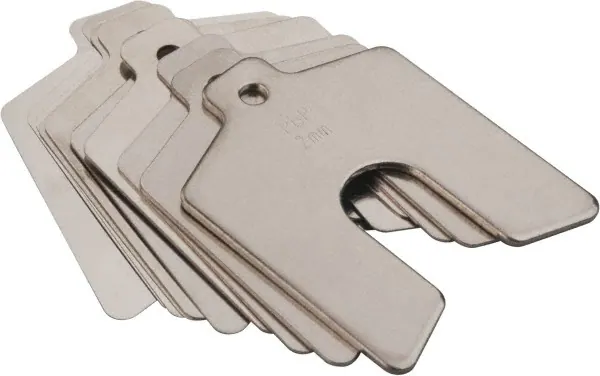
\includegraphics[scale=0.25]{shims.png}
		\captionof{figure}{{\it Shims} of various thicknesses}
		\small\textsuperscript{Source: www.mscdirect.com/product/details/70475967}
		\label{fig:shims}
		
	\end{minipage}\hfill
	\begin{minipage}{0.58\linewidth}
		\scriptsize
		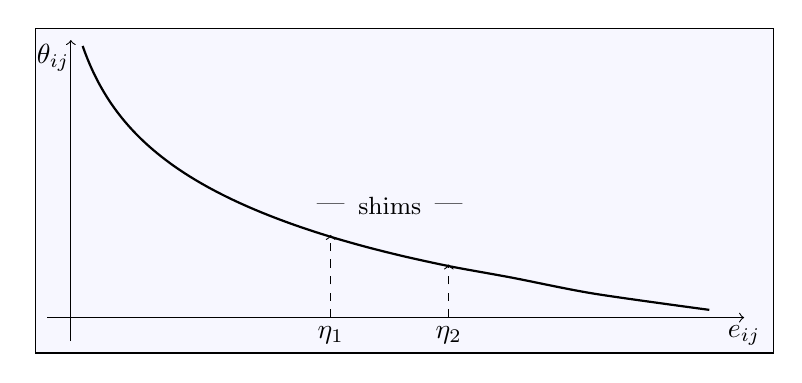
\begin{tikzpicture}[scale=0.75, samples=100]
			\filldraw[fill=blue!3!white, draw=black] (0, 0) rectangle (12.5, 5.5);
			\draw[->] (.2, .6) -- coordinate (x axis mid) (12, .6);
			\node at (5, 0.3) {$\eta_1$};
			\node at (5, 2.5) {|};
			\node at (6, 2.5) {\small{shims}};
			\node at (7, 2.5) {|};
			\node at (7, 0.3) {$\eta_2$};
			\node at (0.3, 5) {$\theta_{ij}$};
			\draw[->] (.6, .2) -- coordinate (y axis mid) (0.6, 5.3);
			\node at (12, 0.3) {$e_{ij}$};
			\draw[smooth, domain = 0.09:2, color=black, thick] plot (.3+1/\x,{4.2+log2(\x)});
			\draw[->, dashed] (5, 0.6)--(5, 2.0);
			\draw[->, dashed] (7, 0.6)--(7, 1.5);
		\end{tikzpicture}
		
		\captionof{figure}{$n_{\pi_k}$\/ possible edges $e_{ij}$\/ sorted by $\theta_{ij}$\/ in non-ascending order}
		\label{fig:whip}		
	\end{minipage}
\end{table}


Considering only the items that can be shipped at the node $\pi_k$, Figure \ref{fig:whip} represents $n_{\pi_k}$\/ possible edges $e_{ij}$\/ of the pallet $i$\/ sorted by $\theta_{ij}$\/ in non-ascending order. Initially, $Shims$\/ builds a greedy solution for the pallet $i$\/ selecting edges up to index $\eta_1$ ({\it greedy phase}). Then, with the edges between $\eta_1$\/ and $\eta_2$, it elaborates different possible complements ({\it composition phase}), including later the best ones in the same pallet ({\it selection phase}). $Shims$\/ is depicted in Algorithm \ref{alg:shims}. 



\begin{algorithm}[H]
	\caption{$Shims$\/ heuristic at node $\pi_k$}  \label{alg:shims}
	\begin{algorithmic}[1]
				
		\State {\bf SolveNode} \,\, {\it in: $Shims, \pi_k, G, tmax, {\color{blue}threshold_1, threshold_2}$} \, \, {\it out: $G(M \cup N_{\pi_k} \cup Q_{\pi_k}, E_{Q_{\pi_k}} \cup E_{N_{\pi_k}})$}
		
		\State $T_{begin} \gets$ current system time
		
		\State Let $G(M \cup N_{\pi_k} \cup Q_{\pi_k}, E_{Q_{\pi_k}})$   \label{shims:initQ}
		
		\State Sort $M$ by $|D_i^{long}|$ in non-descending order \label{shims:pallets}
		
		\State $E_{N_{\pi_k}} \gets \varnothing$ 
		
		\State $\tau_{max} \gets W_{max} \times limit^{CG}_{long}$

		\For{$i \gets 1$ to $m$}  \label{shims:eta1_a}
		
		\State $\tau_{\pi_k} \gets \sum_{(i,q)\in E_{Q_{\pi_k}}} w_q \times D_i^{long}$ 
		\State $vol_i \gets \sum_{(i,q)\in E_{Q_{\pi_k}}} v_q$ 
		
		\State Let $E$\/ be an array of $n_{\pi_k}$ possibles edges of the pallet $i$\/ sorted by $\theta_{ij}$\/ in non-ascending order \label{shims:possible}
		\State $\eta_1 \gets 1$  
		\Repeat
		\State $e_{ij} \gets E_{\eta_1}$ 
		
		\If{ ($E_{N_{\pi_k}} \cup \{e_{ij}\}$ is feasible) {\bf and} ($vol_i \leq V_i \times {\color{blue}threshold_1}$) {\bf and} ($| \tau_{\pi_k} + w_j \times D_i^{long} | \leq W_{max} \times limit^{CG}_{long}$)} 
		
		\State $E_{N_{\pi_k}} \gets E_{N_{\pi_k}} \cup \{e_{ij}\}$
		
		\State $vol_i \gets vol_i + v_j$
		
		\State $\tau_{\pi_k} \gets \tau_{\pi_k} + w_j \times D_i^{long}$
		
		\State $\eta_1 \gets \eta_1 + 1$ 
		
		\EndIf
		\Until ($vol_i > V_i \times {\color{blue}threshold_1}$) {\bf or} ($\eta_1>n_{\pi_k}$) \label{shims:endfirst}	
		
		\State $slack_i \gets V_i - vol_i$  \label{shims:beginsecond}
		\State $\eta_2 \gets \eta_1$  \label{shims:eta2a}
%		\While{($\eta_2 \leq n_{\pi_k}$) {\bf and} ($ vol_i < (1 + 2 \times (1-limit)) \times V_i$)}
{\color{blue}
		\While{($\eta_2 \leq n_{\pi_k}$) {\bf and} ($ vol_i < V_i \times {\color{blue}threshold_2}$)}
	
		\State $e_{ij} \gets E_{\eta_2}$
		
		\State $vol_i \gets vol_i + v_j$
		\State $\eta_2 \gets \eta_2 + 1$  \label{shims:eta2} 
		\EndWhile \label{shims:endsecond} 
	}
		\State $vol \gets 0$; $b \gets 1$; $shims_b \gets \varnothing$; $Set \gets \{ shims_b \}$  \label{shims:beginthird} 
				
		\For{$x \gets \eta_1$ to $\eta_2$} \label{edges_indexes}
		
		\If{ $T_{current} - T_{begin} > tmax$}
		\State {\bf break}
		\EndIf
		
		\State $NewShims \gets$ {\bf True} \label{new_shims}
		\State $e_{ij} \gets E_x$
		
		\For{$shims \in Set$} \label{shims_set}
		
		\If {($e_{ij} \not\in (E_{N_{\pi_k}} \cup shims))$ {\bf and} ($e_{ij}$ is feasible)  {\bf and} ($(v_j + vol) \leq slack_i$)}
		
		\State $shims \gets shims \cup \{e_{ij}\}$
		\State $vol \gets vol + v_j$
		\State $NewShims \gets$ {\bf False} \label{new_shims_false}
		
		\State {\bf break}  
		\EndIf
		
		\EndFor 
		
		\If{$NewShims$} \label{new_shims2}
		\State $vol \gets 0$; $b \gets b + 1$;  $shims_b \gets \{e_{ij}\}$
		\State $Set \gets Set \cup \{ shims_b \}$
		\EndIf
		
		\EndFor 
		
		\State $sh_w \gets shims$, where $shims \in Set$ and $\sum_{e_{ij} \in shims} w_j$\/ is maximum  \label{best_weight}		
		\State $sh_v \gets shims$, where $shims \in Set$ and $\sum_{e_{ij} \in shims} v_j$\/ is maximum \label{best_volume}
		\State $sh_{best} \gets shims$, where $shims \in \{sh_w, sh_v\}$\/ and $\sum_{e_{ij} \in shims} s_j$\/ is maximum \label{best_score}
		\State $E_{N_{\pi_k}} \gets E_{N_{\pi_k}} \cup sh_{best}$ \label{shims:endthird}  
		
		\EndFor

	\end{algorithmic}
\end{algorithm}

{\color{blue}The arguments $threshold_1$ and $threshold_2$ are the volume thresholds for $\eta_1$ and $\eta_2$ calculations, respectively.

The argument $tmax$ is the maximum time for Shims to solve a node. It is proportional to the sum of the candidate items volumes in each node, in relation to the sum of all nodes $tmax$, and the maximum time to solve the tour.

}

Initially, $Q_{\pi_k}$\/ (line \ref{shims:initQ}) corresponds to the packed contents that remain on board. It is important to remember that $E_{Q_{\pi_k}}$\/ and $M$\/ were modified by the procedure $UpdatePacked(M, Q_{\pi_k}, \pi_k)$ and the procedure $SetPalletsDestinations(M, \pi_k)$. Then, the pallets $i$\/ are considered in non-descending order of $|D_i^{long}|$.

For each pallet $i$, its $n_{\pi_k}$\/ possible edges $e_{ij}$\/ are considered in non-increasing order of $\theta_{ij}$:

\begin{itemize}
	
	\setlength\itemsep{-0.3em}
	
	\item In the {\it greedy phase}\/ (lines \ref{shims:pallets}-\ref{shims:endfirst}), a partial solution for each pallet $i$\/ is constructed by adding edges following $\theta_{ij}$\/ order.
	The $\eta_1$\/ index corresponds to the accumulated volume equal to $V_i \times {\color{blue}threshold_1}$. In $\eta_2$\/ index, this same accumulated volume reaches $V_i \times  {\color{blue}threshold_2}$. {\color{blue}The values of these thresholds were defined empirically by the {\it iRace}\/ tool \citep{LopezIbanezManuel2016}}.
	
	\item In the {\it composition phase}\/ (lines \ref{shims:beginsecond}-\ref{shims:endsecond}), a set of shims named $Set$\/ is created for each pallet $i$, where each shim is formed by a set of edges in the range $[\eta_1,\eta_2]$, whose total volume is limited by $slack_i$. In this phase, the heuristic that provided the best results, both in terms of time and quality, is based on {\it First-Fit Decreasing}, which is an approximation algorithm for the {\it Bin Packing Problem}\/ \citep{JohnsonGarey1985}. Basically, shims are created by accumulating the following edges, taking $slack_i$\/ as a limit.
	
	\item In the {\it selection phase}\/ (lines \ref{shims:beginthird}-\ref{shims:endthird}), the best shim in $Set$\/ is chosen. Initially, two shims are found: $sh_w$\/ with larger weight and $sh_v$\/ with larger volume. Between the two, the one with the highest score will be chosen, and its edges will be inserted into $E_{N_{\pi_k}}$.
	
\end{itemize}

{\color{blue}
	iRace (Iterated Racing for Automatic Algorithm Configuration) streamlines the tuning of optimization algorithms by iteratively testing and eliminating weaker parameter configurations through statistical comparisons. It focuses computational resources on the most promising settings. This method significantly cuts down the time and effort needed to find optimal or near-optimal parameters, proving effective across various application domains.
}


\section{Implementation and results}
\label{results}

This section is composed of two parts: the generation of the test instances and the results obtained in our implementation.


\subsection{Instances generation}
\label{items}

As we are dealing with a new problem that until now had not been modelled in the literature, we have to create our own benchmarks. For this, we based it on the characteristics of real airlifts carried out by the {\it Brazilian Air Force}, as described below.

In the delivery of supplies carried out in Brazil from 2008 to 2010, 23\% of the items weighed between $10kg$ and $20kg$, 22\% from $21kg$ to $40kg$, 24\% from $41kg$ to $80kg$, 23\% from $81kg$ to $200kg$, and 8\% between $201kg$ and $340kg$. These five groups of items are described in Table \ref{tab:weights}, where $P$\/ represents the group probability. On the other hand, the average density of these items is approximately $246 kg/m^3$.

\begin{table}[h]
	\centering
	\caption{Items weight distribution}  \label{tab:weights}
	\begin{tabular}{c c c c }
		\toprule
		$x$ & $P$ & $low$ ($kg$) & $high$ ($kg$) \\		
		\midrule
		1              & 0.23           & 10  & 20  \\
		2              & 0.22           & 21  & 40  \\
		3              & 0.24           & 41  & 80  \\		
		4              & 0.23           & 81  & 200 \\
		5              & 0.08           & 201 & 340 \\
		\bottomrule
	\end{tabular}
\end{table}


In the generation of test instances, we use two types of random selections:
\begin{itemize}
	\setlength\itemsep{-0.3em}
	\item $RandomInt(i_1,i_2)$: randomly selects a integer number in $[i_1,i_2]$, where $i_1$ and $i_2$ are integer numbers;
	\item $Roulette(set)$ biased through $\phi$: selects an element from $set$, where the probability of each element is proportional to the value of a given function $\phi$\/ defined on $set$.
\end{itemize}

The procedure $ItemsGeneration$, which generates $N$ (all items to be moved among the nodes), is described in Algorithm \ref{alg:itemsgen}.


\begin{algorithm}[H]
	\caption{Generating items}  \label{alg:itemsgen}
	\begin{algorithmic}[1]
		\State {\bf ItemsGeneration} \,\, {\it in: $scenario, surplus$} \, \, {\it out: $N$}
		\State Let $L$ be the set of nodes and $M$ the set of pallets  \label{ig:LM}
		\State $limit \gets surplus \times \sum_{i=1}^{m} V_i$ \label{ig:extended}
		\For{$k \gets 0$ to $K$}
		\State $N_k \gets \varnothing$
		\State $j \gets 0$
		\State $vol \gets 0$	\label{ig:totals}	
		\While{$vol < limit$}
		\State $j \gets j+1$
		\State Let $t_j^k$\/ be the item $j$\/ at the node $k$
		\Repeat
		\State $to_j \gets RandomInt(0, K)$ \label{ig:dest}
		\Until{$to_j \neq k$}
		\State $x = Roulette()$ \Comment{biased through $P$ ({\it cfr.} Table \ref{tab:weights})} \label{ig:weight1} 
		\State $w_j \gets RandomInt(low(x), high(x))$        \label{ig:weight2}		
		\State $s_j \gets \round{100 \times (1 - \log_{10}(RandomInt(1, 9)))} $ \label{ig:score}
		\State $v_j \gets w_j / RandomInt(148, 344)$ \label{ig:volume}
		\State $vol \gets vol + v_j$ 
		\State $N_k \gets N_k \cup \{t_j^k\}$ 
		\EndWhile
		\EndFor
		\State $N \gets \bigcup_{0 \leq k \leq K} N_k$
	\end{algorithmic}
\end{algorithm}

$scenario$\/ defines $L$\/ and $M$\/ (line \ref{ig:LM}), and the argument $surplus$\/ sets a limit on the total volume of items at each node (line \ref{ig:extended}). To avoid simply loading all items, we use $surplus \in \{1.2,\ 1.5,\ 2.0\}$\/. This also represents more instances for tests in each scenario.

For each generated $t^k_j$ item, its destination is randomly selected (line \ref{ig:dest}), its weight has a distribution according to Table \ref{tab:weights} (lines \ref{ig:weight1}-\ref{ig:weight2}), its score varies $100$\/ (highest) and $5$\/ (lowest) according to a logarithmic scale (line \ref{ig:score}), and its volume is randomly defined from the density, where we allow a variation of 40\% around the average density of $246 kg/m^3$\/ (line \ref{ig:volume}).


{\color{blue}
	After the items were generated, some experiments with the \textit{iRace} tool were executed to determine the values for parameters $threshold_1$ and $threshold_2$ used in \textit{Shims}, whose results are presented in Table \ref{tab:irace}.
	
	\begin{table}[H]
		\centering
		\caption{\textit{iRace} testing results}  \label{tab:irace}
		\footnotesize
		\begin{tabular}{cccc}
			\toprule
			\textbf{surplus} & \boldm{$threshold_1$} & \boldm{$threshold_2$} & \textbf{time (min)}\\
			\midrule
			1.2& 0.8621 & 1.0539 & 47 \\
			1.5& 0.9199 & 1.1399 & 59 \\
			2.0& 0.9617 & 1.5706 & 63 \\						
			\bottomrule
		\end{tabular}
		\normalsize
	\end{table}
	
	For these tests, we considered the odd instances (1, 3, 5, 7) as the \textbf{training} set and the even instances (2, 4, 6) as the \textbf{testing} set for the \textit{iRace} runs. We supplied \textit{iRace} for $threshold_1$ determination, the range [0.8, 1.0], and for $threshold_2$, the range [1.0, 2.0]. The number of iterations in each experiment was limited to 3000 executions for \textit{iRace} to have plenty of data for its statistical tests. More detail about these configurations may be found on the \textit{iRace} user guide in {\tt cran.r-project.org/web/packages/irace/irace.pdf}.
}


\subsection{Obtained solutions: quality and runtimes}

In the tests performed, we used a 64-bit, 16 GB, 3.6 GHz, eight-core processor with {\it Linux Ubuntu 22.04.1 LTS 64-bit} as the operational system and {\it Python 3.10.4}\/ as the programming language. We also used the well-known solver $Gurobi$\/ ({\tt www.gurobi.com}), version 9.5.2.

We ran Algorithm \ref{alg:main} considering the five scenarios from Table \ref{tab:scenarios}, three values for  $surplus$\/ from $\{1.2, 1.5, 2.0\}$, four values for $tmax$\/ from $\{240s, 1200s, 2400s, 3600s\}$, and six different $method$\/ for the node-by-node solution: $Gurobi$\/ (see \ref{solver}), ACO, NMO, TS, GRASP, and $Shims$\/ (Algorithm \ref{alg:shims}). 

For $Gurobi$\/ to be able to solve the largest possible number of tests without memory overflow, we set its parameter {\it MIPgap}\/ to 1\%. This shortens its runtime, in addition to ensuring that its objective function $f$\/ is at most 1\% of the optimal solution. For more details, see {\tt www.support.gurobi.com}.

	
\begin{table}[H]
{\color{blue}
	\centering
	\caption{Overall results}  \label{tab:mr}
	\footnotesize
	\begin{tabular}{cccc}	
	\toprule
	{\bf Method} & {\bf Best scenarios} & {\bf Worst scenarios} & {\bf Worst run times (min)}  \\
	\midrule
	NMO           & 4             & 5    & {\color{red}60}  \\
	ACO           & 2, 3          & 4, 5 & {\color{red}25}, {\color{red}61}  \\
	GRASP         & 1             & 4, 5 & {\color{red}28}, {\color{red}55}  \\
	TS            & -             & 5    & {\color{red}44}  \\
	\midrule
	{\it Gurobi}  & 1, 2, 3, 4    & 5    & {\color{red}did not solve}  \\
	{\it Shims}   & 1, 2, 3, 4, 5 & -    & {\bf 3.26} \\
	\bottomrule
	\end{tabular}
\normalsize
}
\end{table}


\subsubsection{Shims results}

Among the heuristics, we will present only the results obtained by $Shims$, which had the best performance. For each $scenario$, $surplus$\/ and $tmax$, seven different instances were generated. We will present the average of the objective function $f$\/ and the runtime of $Gurobi$\/ and $Shims$\/ in these instances. To facilitate the comparison between both, we added a last column in the tables where two values are indicated:

\begin{itemize}
	\setlength\itemsep{-0.3em}
	\item {\bf Normalized}: value between 0 and 1, which corresponds to the ratio between the sum of $f$\/ values obtained by the method in all scenarios and the sum of the best values obtained by both methods in all scenarios. The higher the value of {\bf Normalized}, the closer the method approached the best solutions found.
	\item {\bf Speed-up}: ratio of the sums of the runtimes of all scenarios and the sum of the method runtimes in all scenarios. The method with the highest {\bf Speed-up}\/ is the fastest.
\end{itemize}


We also indicate the two adopted strategies: dedicating all the processing time to the two shortest tours or distributing it among all $K!$\/ tours.

The results obtained with $tmax = 3600s$, which is the highest tested runtime limit, are in Tables \ref{tab:20}, \ref{tab:50} and \ref{tab:100}, with $surplus$\/ values of $1.2$, $1.5$\/ and $2.0$, respectively. We indicate with an {\bf x} the cases where $Gurobi$\/ did not find a feasible solution within this runtime limit or had to be aborted due to high random-access memory (RAM) usage.



\begin{table}[H]
	\centering
	\caption{Solutions with $surplus = 1.2$\/ and $tmax =  3600s$}  \label{tab:20}
	\footnotesize
	\begin{tabular}{ccccccccc}
		\toprule
		{\specialcell{{\bf Tested}\\{\bf tours}}}&$method$&$scenario$&{\bf 1}&{\bf 2}&{\bf 3}&{\bf 4}&{\bf 5}&\specialcell{{\bf Normalized}\\{\bf Speed-up}}   \\
		\toprule
		\multirow{4}{*}{Shortest} &\multirow{2}{*}{$Gurobi$}  & $f$ & 8.61    & 11.56   & 13.67   & 13.87 & 12.48       &  0.9985 \\ % best 6028
		&                              &               {time (s)}   & 26      & 22      & 28      & 28    & 25          &  1.0    \\ % longer 129
		\cmidrule(lr){2-9}
		&                           \multirow{2}{*}{$Shims$}  & $f$ & 8.61    & 11.56   & 13.46   & 13.93 & 12.51       &  0.9965 \\
		&                             &                {time (s)}   & 1       & 1       & 1       & 1     & 1           &  25.8   \\
		
		\midrule
		
		\multirow{4}{*}{All $K!$}&  \multirow{2}{*}{$Gurobi$} & $f$ & 8.60    & 12.20   & 13.66   & 15.00  & {\bf x}    & 0.9998 \\ % best 4947
		&                              &               {time (s)}   & 30      & 35      & 123     & 314    & {\bf x}    & 1.0 \\
		\cmidrule(lr){2-9}	
		&                           \multirow{2}{*}{$Shims$}  & $f$ & 8.61    & 12.20   & 13.46   & 14.99  & 13.35      & 0.9958  \\
		&                              &               {time (s)}   & 1       & 1       & 4       & 10     & 51         & 7.49   \\
		\bottomrule
		
	\end{tabular}
	\normalsize
\end{table}


\begin{table}[H]
	\centering
	\caption{Solutions with $surplus = 1.5$\/ and $tmax =  3600s$}  \label{tab:50}
	\footnotesize
	\begin{tabular}{ccccccccc}
		\toprule
		{\specialcell{{\bf Tested}\\{\bf tours}}} & $method$          & $scenario$ & {\bf 1} & {\bf 2} & {\bf 3} & {\bf 4} & {\bf 5} & \specialcell{{\bf Normalized}\\{\bf Speed-up}}   \\
		\toprule
		\multirow{4}{*}{ Shortest } & \multirow{2}{*}{$Gurobi$} & $f$ & 11.76 & 16.29 & 18.02 & 19.42 & 16.35 & 0.9994 \\ % best 8189
		&&               {time (s)}                                   & 51    & 39    & 40    & 36    & 38    & 1.0 \\ 
		\cmidrule(lr){2-9}	
		&\multirow{2}{*}{$Shims$}                               & $f$ & 11.78 & 16.29 & 17.96 & 19.43 & 16.37 & 0.9993  \\
		&&         {time (s)}                                         & 1     & 1     & 2     & 2     & 2     & 25.5  \\
		
		\midrule
		
		\multirow{4}{*}{All $K!$} & \multirow{2}{*}{$Gurobi$}   & $f$ & 11.76 & 16.37 & 18.01 & 20.95 & 17.60 & 0.9999 \\  % best 8469
		&&               {time (s)}                                   & 64    & 58    & 195   & 472   & 2258  & 1.0  \\
		\cmidrule(lr){2-9}	
		&\multirow{2}{*}{$Shims$}                               & $f$ & 11.78 & 16.29 & 17.99 & 20.93 & 17.50 & 0.9976  \\ 
		&&         {time (s)}                                         & 1     & 2     & 5     & 15    & 100   & 23.8 \\
		\bottomrule
		
	\end{tabular}
	\normalsize
\end{table}


\begin{table}[H]
	\centering
	\caption{Solutions with $surplus = 2.0$\/ and $tmax =  3600s$}  \label{tab:100}
	\footnotesize
	\begin{tabular}{ccccccccc}
		\toprule
		{\specialcell{{\bf Tested}\\{\bf tours}}}& $method$& $scenario$ & {\bf 1} & {\bf 2} & {\bf 3} & {\bf 4} & {\bf 5} & \specialcell{{\bf Normalized}\\{\bf Speed-up}}   \\
		\toprule
		\multirow{4}{*}{Shortest} & \multirow{2}{*}{$Gurobi$} & $f$ & 17.89 & 24.96 & 26.15 & 27.52 & 23.85 & 0.9996 \\ % best 12042
		&&                                              {time (s)}  & 183   & 87    & 73    & 79    & 71    & 1.0  \\
		\cmidrule(lr){2-9}	
		&                            \multirow{2}{*}{$Shims$} & $f$ & 17.94 & 24.96 & 26.03 & 27.43 & 23.73 & 0.9972  \\
		&&                                              {time (s)}  & 1     & 2     & 2     & 3     & 4     & 41.1  \\
		
		\midrule
		
		\multirow{4}{*}{All $K!$} & \multirow{2}{*}{$Gurobi$} & $f$ & 17.90 & 25.44 & 26.15 & 29.13 &{\bf x}& 0.9994 \\ % best 9867
		&&                                               {time (s)} & 178   & 143   & 378   & 862   &{\bf x}& 1.0  \\
		\cmidrule(lr){2-9}	
		&                         \multirow{2}{*}{$Shims$}    & $f$ & 17.94 & 25.45 & 26.14 & 28.84 & 26.22  & 0.9970  \\
		&&                                               {time (s)} & 1     & 3     & 10    & 31    & 196    & 34.7  \\
		\bottomrule
		
	\end{tabular}
	\normalsize
\end{table}


From these data, we can draw some conclusions:

\begin{itemize}
	\setlength\itemsep{-0.3em}
	\item The strategy of testing all $K!$\/ tours often provide a better-quality solution, even with less time on each node. This shows that the four sub-problems are interconnected in such a way that it is not enough to solve them separately.
	\item $Gurobi$\/ fails in some cases when $scenario=5$\/ and the strategy is to check all $K!$\/ tours. This occurs because the runtime limit per node is smaller and there tend to be more packed contents on the aircraft, reducing the space for allocating items and making the solution difficult.
	\item When $Gurobi$\/ finishes, it finds the best solution, but the one obtained by $Shims$\/ reaches {\color{blue}$99.9\%$}\/ of that value.
	\item $Shims$\/ always finds a solution, being {\color{blue}8 to 41} times faster.
	\item All runtimes are much lower than the limit because the solution on many nodes can be fast. Anyway, in all the tests performed, the maximum time spent by $Shims$\/ did not reach 4 minutes. On the other hand, when $scenario=5$\/ and $surplus=1.5$, $Gurobi$\/ spent almost 40 minutes.
\end{itemize}

Table \ref{tab:100time} shows the results obtained with the strategy of testing the $K!$\/ tours in all scenarios with different $tmax$. We can observe more cases where $Gurobi$\/ fails, even in smaller scenarios. When $Gurobi$\/ finishes, $Shims$\/ finds a solution of similar quality ($99\%$\/ or better). In all cases, $Shims$\/ finds a good solution in less than 4 minutes.


\begin{table}[H]
	\centering
	\caption{Solutions testing all $K!$\/ tours with different runtime limits}  \label{tab:100time}
	\scriptsize
	\setlength{\tabcolsep}{3.5pt}
	\begin{tabular}{ccc|ccccc|ccccc|ccccc}
		\toprule
		&             \multicolumn{2}{r}{$surplus$} &\multicolumn{5}{c}{\bf 1.2}&\multicolumn{5}{c}{\bf 1.5}&\multicolumn{5}{c}{\bf 2.0} \\
		\midrule
		$method$& {$tmax$} & $scenario$  &{\bf 1}&{\bf 2}&{\bf 3}&{\bf 4}&{\bf 5}&{\bf 1}&{\bf 2}&{\bf 3}&{\bf 4}&{\bf 5}&{\bf 1}&{\bf 2}&{\bf 3}&{\bf 4}&{\bf 5} \\
		\toprule
		
		\multirow{10}{*}{$Gurobi$} & \multirow{2}{*}{240s} & $f$ & 8.60 & 12.20 & 13.67 & {\bf x} & {\bf x} & 11.77 & 16.38 & 18.10 & {\bf x} & {\bf x} & 17.89 & 25.42 & {\bf x} & {\bf x} & {\bf x} \\ 
		&               &  {time (s)}                            & 31   & 35    & 124   & {\bf x} & {\bf x} & 52    & 59    & 200   & {\bf x} & {\bf x} & 188   & 145   & {\bf x} & {\bf x} & {\bf x} \\ 
		\cmidrule(lr){2-18}		
		
		&                           \multirow{2}{*}{1200s} & $f$ & 8.61 & 12.20 & 13.31 & 10.00   & {\bf x} & 11.77 & 17.02 & 18.25 &  20.64  & {\bf x} & 17.75 & 25.24 & 26.49 & 27.97   & {\bf x} \\ 
		&        &  {time (s)}                                   & 28   & 37    & 129   & 320     & {\bf x} & 46    & 61    & 190   &  304    & {\bf x} & 161   & 139   & 384   & 579     & {\bf x} \\ 
		\cmidrule(lr){2-18}                              
		&                           \multirow{2}{*}{2400s} & $f$ & 8.60 & 12.21 & 13.67 & 15.00   & 13.41   & 11.77 & 16.37 & 18.03 & 20.95   & {\bf x} & 17.89 & 25.44 & 26.15 & 29.13   & {\bf x} \\
		&        &  {time (s)}                                   & 26   & 38    & 134   & 310     & 1520    & 46    & 60    & 199   & 461     & {\bf x} & 164   & 140   & 383   & 786     & {\bf x} \\
		\cmidrule(lr){2-18}                              		
		
		&                           \multirow{2}{*}{3600s} & $f$ & 8.60 & 12.20 & 13.66 & 15.00   & {\bf x} & 11.76 & 16.37 & 18.01 &  20.95  & 17.60   & 17.90 & 25.44 & 26.15 & 29.13   & {\bf x} \\ 
		&        &  {time (s)}                                   & 30   & 35    & 123   & 314     & {\bf x} & 64    & 58    & 195   &  472    & 2258    & 178   & 143   & 378   & 862     & {\bf x} \\ 
		
		\midrule
		
		\multirow{2}{*}{$Shims$} &  \multirow{2}{*}{240s}  & $f$ & 8.61 & 12.20 & 13.46 & 14.99   & 13.35   & 11.78 & 16.29 & 17.99 &  20.93  & 17.50   & 17.94 & 25.45 & 26.14 & 28.84   & 26.22 \\ % 
		&         & {time (s)}                                   & 1    & 2     & 4     & 10      & 51      & 1     & 2     & 5     &  15     & 100     & 1     & 3     & 10    & 31      & 196   \\ 
		
		\bottomrule
	\end{tabular}
	\normalsize
\end{table}

The actual RAM consumption of $Gurobi$\/ was over 8.5 GB, and all of $Shims$\/'s executions consumed at most 1.5 GB of RAM.

{\color{blue}
\subsection{{\it Shims} validation with more nodes}

To validate the effectiveness of the {\it Shims} heuristic, we solve a 15-node TSP containing the 15 main Brazilian airports.
For this task, we implemented a TSP solution method based on the Genetic Algorithm (GA) that returns the 20\% best tours as input to the ACLP-RPDP solved by {\it Shims}.

We implemented the GA with DEAP (Distributed Evolutionary Algorithms in Python) , a evolutionary computation framework available in {\tt github.com/deap/deap}. More details can be found in \citep{DEAP_JMLR2012}.

DEAP took 3 seconds to solve a 15-node TSP.

\citep{PeerlinckAmy2022MFEO} applied DEAP to solve a Multi-Objective Knapsack Problem. This algorithm is adapted to solve the ACLPP in each node of this work's solution.

}

\section{Conclusions}
\label{conclusions}

In this work, we modelled and solved a real air transport problem named {\it Air Cargo Load Planning with Routing, Pickup, and Delivery Problem}\/ (ACLP+RPDP). For the first time in the literature, a {\it NP-hard}\/ problem that involves {\it simultaneously}\/ pallet assembly, load balancing, and route planning is addressed, where the cost-effectiveness of transport is maximized. Currently, there is no commercial software available for this problem.

We adopted some simplifications that are not critical, but that allowed for an unprecedented solution to this problem considering more than two nodes. In practical cases, the number $K$\/ of nodes, excluding the base, is small ($K \leq 6$), each of which has hundreds of items to be shipped. Considering a real aircraft, we have developed some node-by-node solutions. This allows us to test two strategies: find a solution using the shortest tours, or enumerate all $K!$\/ tours and choose the best. The complete process can be executed quickly on a handheld computer, offering good results and reducing stress for the transport planners.

As validation, we carried out tests in several real air transport scenarios. In these cases, the solution process can establish, in less than four minutes, a flight tour for a single aircraft with a good distribution of load on pallets to be put in the cargo bay, enforcing the loaded aircraft balance, maximising the total score, and minimising fuel consumption along the planned route, which is beneficial to reduce carbon emissions. This output is an essential part of airlift: it guarantees flight safety, makes ground operations more efficient, and makes sure that each item gets to its right destination.

Our main contributions were the mathematical modelling of ACLP+RPDP, involving four well-known and interconnected {\it NP-hard}\/ sub-problems, a complete process to solve it, and a new heuristic named {\it Shims}\/ that offers fast node solutions with good quality. The method of this work is not exclusive to aircraft and airports: it can be adapted to ships and ports, vehicles and warehouses, or wagons and railways, provided that their practical cases are similar to those considered here. In these situations, it would be necessary to make some changes in the model: for example, modify the load balancing constraints and consider the available space in vehicles or wagons instead of pallets.

Because we applied this heuristic process to all $K!$\/ tours, perhaps it seems that our methodology is not generalizable. This is not true; we did this because {\it Shims}\/ is very fast and $K$\/ is small in practical cases of air transport. In other contexts where $K$\/ may have larger values, this heuristic process remains valid. It is enough to apply it only to some tours that offer a better expectation of a good result, for example, on the TSP's shortest path or other similar ones.

As this is ongoing research, we thought about some possible future improvements: consider more than one aircraft, implement parallel algorithms in some steps of the solution to improve computational efficiency, and model 3-D items.


\section*{CRediT authorship contribution statement}

\textbf{Antonio Celio Pereira de Mesquita:} Conceptualization, Methodology, Software, Writing - original draft preparation, Investigation, Validation. \textbf{Carlos Alberto Alonso Sanches:} Conceptualization, Methodology, Resources, Supervision, Writing - reviewing \& editing.

\section*{Declaration of competing interest}

The authors declare that they have no known competing financial interests or personal relationships that could have appeared to influence the work reported in this paper.

\section*{Data availability}

The dataset and code used in this work are available in {\tt github.com/celiomesquita/ACLP\_RPDP\_P}.

\section*{Acknowledgments}

This research was partially supported by the S\~{a}o Paulo Research Foundation (FAPESP), grant 2022/05803-3.


\section*{References}

\bibliographystyle{apalike} 

\bibliography{bib}


\end{document}
